
%======================================================================
% GÓI 1 (VIẾT LẠI): MỞ ĐẦU VÀ BẰNG CHỨNG VĨ MÔ VỀ "NGHỊCH LÝ PHÁT TRIỂN"
% (Phần 1: Tăng trưởng và Thành tựu)
%======================================================================

\chapter{越南外部质量保障体系现状分析}
\label{chap:thuc_trang}

\section*{引言}
\addcontentsline{toc}{section}{引言}

本章将对越南高等教育(GDĐH)外部质量保障(ĐBCL)体系的现状进行深入和多维度的分析,重点关注2015年至2024年这一强劲转型阶段。本章将运用第二章所论证的V-AQA理论模型视角,重点“解剖”一个深刻的\textbf{发展悖论(development paradox)}:即规模和投入指标的爆炸性增长,并未伴随着产出质量及与劳动力市场契合度的相应提升。

通过综合分析宏观统计数据、世界银行等权威国际组织的报告、学术研究,特别是通过图表进行可视化的数据,本章将提供坚实的科学论据。目标不仅是描述现状,更是要解释阻碍质量提升努力的系统性“瓶颈”和“恶性循环”。从而,本章将为后续章节提出战略性解决方案奠定坚实的实践基础。

\section{越南高等教育中的发展悖论}
\label{sec:nghich_ly_phat_trien_vimo}

2015-2024年阶段标志着越南高等教育一个充满变动的转型历程,揭示了一个深刻的发展悖论。一方面,该体系在教育大众化、扩大培养规模以及提升投入资源质量方面取得了前所未有的成就。另一方面,这些关于“量”的成就,却掩盖了关于“质”的持续挑战,体现在毕业生技能与劳动力市场实际需求之间日益扩大的不匹配。分析此悖论的两个方面,是理解该体系核心挑战的先决条件。

\subsection{悖论的第一面:规模的爆炸性增长与投入资源的改善}
\label{subsec:ve_thu_nhat_nghich_ly}

不可否认,越南高等教育在扩大民众教育机会方面取得了令人瞩目的进展。这一时期见证了强劲的大众化进程,体现在办学机构网络的拓展和学生规模的飞跃式增长。

\subsubsection{拓展教育网络与培养规模}

过去十年越南高等教育体系发展的全貌,通过图\ref{fig:so_truong_quy_mo_sv}得以清晰展现。

\begin{figure}[h!]
    \centering
    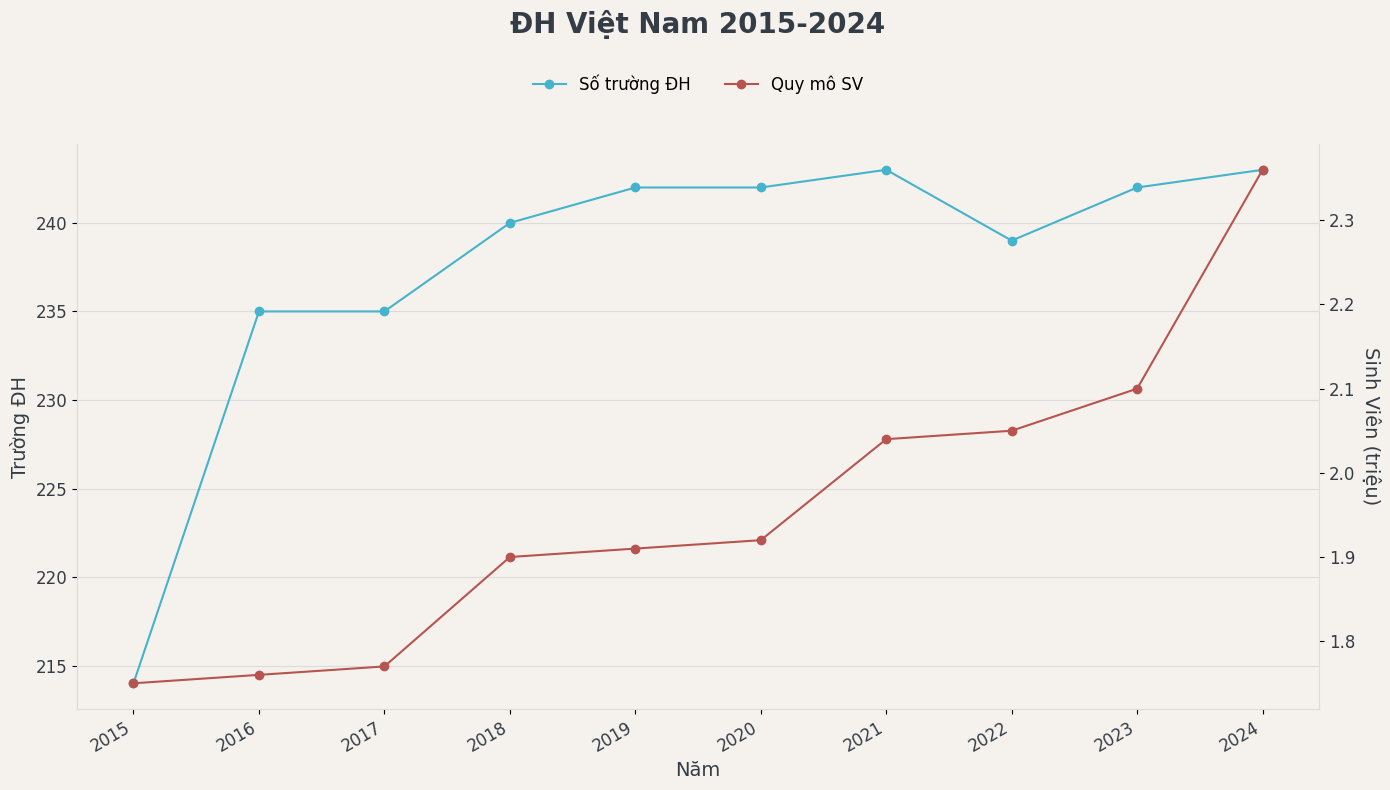
\includegraphics[width=\textwidth]{image/dh_viet_nam_2015_2024.png}
    \caption{越南高等教育办学机构数量与学生规模发展情况(2015-2024年)}
    \label{fig:so_truong_quy_mo_sv}
\end{figure}

分析图\ref{fig:so_truong_quy_mo_sv}显示了两种同步但速度不同的增长趋势。
\begin{itemize}
    \item \textbf{关于网络(蓝色线):} 高等教育机构数量呈现稳定而坚实的增长趋势,从2015年的215所增至2024年的243所。这一增长虽然不算突变,但反映了政府在拓展办学机构网络方面的一贯政策,包括成立新大学和升级专科学校,旨在为全国民众提供多样化的学习机会。
    \item \textbf{关于学生规模(红色线):} 与学校数量的平稳增长形成对比的是,学生规模呈现出异常强劲的爆炸性增长。在经历了2015年至2021年的相对稳定期后,学生规模在最后三年(2022-2024)内从约205万猛增至超过\textbf{235万学生}。这一飞跃不仅体现了高等教育日益增长的吸引力,也表明该体系正承受着为前所未有的大量学生提供培养需求的巨大压力。
\end{itemize}

这一增长正逐步使越南更接近到2030年实现\textbf{每万人口260名大学生}的国家战略目标\footcite{sggp_en_3million_2030}。此外,它还体现在重要的国际指标——高等教育毛入学率(GER)上。世界银行和联合国教科文组织的数据显示,越南的毛入学率已从2000年的仅10.3\%飙升至2018年的28.6\%,并于\textbf{2022年达到创纪录的42.22\%}\footcite{worldbank_humancapital_2022}。这是一项值得称道的成就,显示了教育大众化政策的成功。

\subsubsection{改善投入资源质量}
在扩大规模的同时,该体系的投入资源质量也取得了显著改善,显示了在提升内在能力方面的有目的的投资。
\begin{itemize}
    \item \textbf{师资队伍质量:} 拥有研究生学历(硕士或博士)的大学教师比例几乎翻了一番,从2007年的47\%增至\textbf{2020年达到85\%}\footcite{worldbank_p178112}。对提升师资队伍水平的投资是一个基础性因素,有望直接转化为教学和研究质量。
    \item \textbf{科学研究能力:} 提升教师水平的成就已产生具体影响。越南人均在国际权威期刊上可引用的科学文献数量,在十年间(2010-2020)\textbf{增长了三倍}\footcite{worldbank_improvingperformance_2020}。这表明该体系的研究能力取得了飞跃式进展,正逐步与国际科学界接轨。
\end{itemize}

上述数字和图表描绘了一幅关于悖论第一面的乐观画面:一个正在强劲发展、在网络、学生规模乃至投入资源质量等各方面都在扩张的高等教育体系。这些是不可否认的成就,为一个现代化和国际化的高等教育体系奠定了坚实的基础。然而,这幅画面只是一个更为复杂的悖论的一半。当我们将这些关于“量”的成就与关于产出质量和体系效率的指标进行对比时,一个充满挑战和警示的另一面故事开始显现。悖论的第二面将在下一部分深入分析。



% het goi 1



